\documentclass[a4paper,11pt]{scrartcl} 
\usepackage{geometry} 
\geometry{left=2.5cm} \geometry{top=3cm}

\usepackage[utf8]{inputenc} 
\usepackage[ngerman]{babel} 
\usepackage[T1]{fontenc} 
\usepackage{amsmath} 
\usepackage{amssymb} 
\usepackage[onehalfspacing]{setspace} 
\usepackage{graphicx} 
\usepackage{epstopdf} 
\usepackage{csquotes} 
\usepackage{array} 
\usepackage{upgreek} 
\usepackage{float} 
\usepackage{tikz} 
\usepackage[font=small]{caption}
\usepackage[backend=biber, style=chem-angew]{biblatex} 
\addbibresource{Blatt 7.bib} 
\usepackage{tabularx, booktabs, multirow} 
\usepackage{listings}
\usepackage{chemgreek}
\usepackage{chemformula}
\captionsetup{format=plain}
%\usepackage{hyperref}
\usepackage[hidelinks]{hyperref}
\usepackage{svg}
\usepackage{subcaption}
\usepackage{siunitx}
\sisetup{detect-weight=true, detect-family=true,locale=DE,range-phrase={\,bis\,},list-final-separator ={\,\linebreak[0] \text{und}\,},separate-uncertainty=true,per-mode = symbol-or-fraction}

\parindent0pt %Kein Einzug am Anfang von Absätzen
\sloppy %Besserer Blocksatz
%\renewcaptionname{ngerman}{\figurename}{Abb.} 
%\renewcaptionname{ngerman}{\tablename}{Tab.} 
\setkomafont{section}{\normalsize}

\lstset{
    language=Python,
    numbers=left,
    numberstyle=\tiny\color{gray},
    numbersep=8pt,
    stepnumber=1,
    frame=single,
    tabsize=4,
    showstringspaces=false,
    breaklines=true,
    keywordstyle=\color{blue}\bfseries,
    stringstyle=\color{red},
    commentstyle=\color{green!50!black},
    basicstyle=\ttfamily\small,
    literate={ö}{{\"o}}1
             {ä}{{\"a}}1
             {ü}{{\"u}}1
             {ß}{{\ss}}1
}

\title{Blatt 11}
\author{Vincent Kümmerle und Elvis Gnaglo}
\date{\today}

\begin{document}

\maketitle

\section{Erstellen einer Vektorgrafik}
Die Vektorgrafik zur Brechung eines Laserstrahls an einem Prisma wurde mit Inkscape erstellt. Die einzelnen Schritte sind in den folgenden Abbildungen dargestellt.

\begin{figure}[H]
    \centering
    \begin{subfigure}[b]{0.49\textwidth}
        \centering
        \includegraphics[width=\textwidth]{Bilder/Screenshot 2026-01-06 114503.png}
        \caption{Erstellung des Dreiecks mit Polygon-Werkzeug.}
        \label{fig:bild1}
    \end{subfigure}
    \begin{subfigure}[b]{0.49\textwidth}
        \centering
        \includegraphics[width=\textwidth]{Bilder/Screenshot 2026-01-06 115313.png}
        \caption{Erstellung des Laserstrahls.}
        \label{fig:bild2}
    \end{subfigure}
\end{figure}

\begin{figure}[H]
    \centering
    \begin{subfigure}[b]{0.49\textwidth}
        \centering
        \includegraphics[width=\textwidth]{Bilder/Screenshot 2026-01-06 121853.png}
        \caption{Hinzufügen der gebrochenen Strahlen mit dem Bezier-Werkzeug und des Winkels als Text.}
        \label{fig:bild1}
    \end{subfigure}
    \begin{subfigure}[b]{0.49\textwidth}
        \centering
        \includegraphics[width=\textwidth]{Bilder/Screenshot 2026-01-06 123015.png}
        \caption{Erstellung des Einfalls- und Ausfallslots.}
        \label{fig:bild2}
    \end{subfigure}
\end{figure}
Im letzten Schritt wurde die Seitengröße an den Rahmen um alle Objekte angepasst und die Grafik als PDF exportiert.
\begin{figure}[H]
    \centering
    \includegraphics[width=0.8\textwidth]{Bilder/Screenshot 2026-01-06 131836.png}    
    \caption{Anpassung der Seitengröße an den Rahmen um alle Objekte.} 
\end{figure}

Die erstellte Vektorgrafik ist in Abbildung \ref{fig:Prisma} dargestellt.
Sie zeigt die Brechung eines Laserstrahls an einem Prisma mit dem Einfallswinkel $\alpha$, dem Einfalls- und Ausfallslot sowie den gebrochenen Strahlen im Prisma.
\begin{figure}[H]
    \centering
    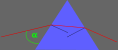
\includegraphics[width=0.8\textwidth]{Bilder/Lichtbrechung.pdf}    
    \caption{Strahlengang eines Laserstrahls an einem Prisma mit Einfallswinkel $\alpha$.}
    \label{fig:Prisma} 
\end{figure}


\section{}

\begin{lstlisting}

\end{lstlisting}


\end{document}